\documentclass[9pt,aspectratio=169]{beamer}

% --- Theme ---
\usetheme{Singapore}
\setbeamertemplate{navigation symbols}{}   % no icons
\setbeamertemplate{mini frames}{}          % no dots in headline
\setbeamercovered{transparent}

% --- Grayscale colors ---
\definecolor{PelloGrayDark}{RGB}{60,60,60}
\definecolor{PelloGray}{RGB}{120,120,120}
\definecolor{PelloGrayLight}{RGB}{235,235,235}
\definecolor{PelloGrayUltraLight}{RGB}{248,248,248}

\usecolortheme[named=PelloGrayDark]{structure}

% --- Blocks ---
\setbeamertemplate{blocks}[rounded][shadow=false]
\setbeamercolor{block title}{fg=white,bg=PelloGrayDark}
\setbeamercolor{block body}{fg=black,bg=PelloGrayLight}
\setbeamercolor{block title example}{fg=white,bg=PelloGrayDark}
\setbeamercolor{block body example}{fg=black,bg=PelloGrayLight}
\setbeamercolor{section in head/foot}{fg=PelloGray,bg=PelloGrayLight}
\setbeamercolor{subsection in head/foot}{fg=PelloGray,bg=PelloGrayLight}
\setbeamercolor{frametitle}{fg=black}

% --- Itemize bullets (optional; keep if you like the style) ---
\setbeamertemplate{itemize item}{\raisebox{0.2em}{\scalebox{.6}{$\bullet$}}}
\setbeamertemplate{itemize subitem}{\raisebox{0.2em}{\scalebox{1}{$-$}}}

% --- Footer: frame numbers ---
\makeatletter
\setbeamertemplate{footline}{%
  \hfill\usebeamerfont{footline}\insertframenumber/\inserttotalframenumber\hspace{1em}\vspace{2pt}
}
\makeatother

% --- Minimal packages (add more only when needed) ---
\usepackage[english]{babel}
\usepackage[T1]{fontenc}
\usepackage[utf8]{inputenc}
\usepackage{graphicx}
\usepackage{tikz}
\usepackage{booktabs}
\usepackage{makecell} % for jumping lines within cells in tables.
\usepackage{multirow}
\usepackage{amsmath}
\usepackage{hyperref}
\hypersetup{colorlinks,linkcolor=,urlcolor=blue}
\usepackage{comment}
\usepackage{listings}
\lstset{
  language=R,
  basicstyle=\ttfamily\footnotesize,
  keywordstyle=\color{blue},
  commentstyle=\color{green!50!black},
  stringstyle=\color{red},
  frame=single,
  showstringspaces=false
}
\linespread{1.7}   % 1.0 = normal, 1.2–1.5 common
\AtBeginEnvironment{lstlisting}{\linespread{1}\selectfont} % keep code listings single-spaced

% Figures: pages of w1_graphs.pdf, built by w1_figures.R from w1_code.R in ../AE_week01_Intro (copy it here after rebuilding)
\newcommand{\graphfig}[1]{\includegraphics[width=0.9\linewidth,page=#1]{w1_graphs.pdf}}

% --- Meta ---
\title{Applied Economics}
\subtitle{Data and Plotting}
\author{Pello Aspuru}
%\institute{University of Vienna}
\date{Winter 2026/2027}

% --- Title page spacing + bottom-left author/date ---
\setbeamertemplate{title page}{
  \vspace{8em}
  \begin{center}
	{\usebeamerfont{title}\inserttitle\par}
  	\vspace{1.5em} % <-- increase title–subtitle gap
  {\usebeamerfont{subtitle}\insertsubtitle\par}
  \end{center}
  \vspace{4em}
  \begin{flushleft}
    {\usebeamerfont{author}\insertauthor\par}
    {\usebeamerfont{date}\insertdate}
  \end{flushleft}
}

\begin{document}

% Title slide without headline/footer
{
  \setbeamertemplate{headline}{}
  \setbeamertemplate{footline}{}
  \begin{frame}
    \titlepage
  \end{frame}
}

\section{Intro}

\begin{frame}{Introduction}
  Previous sessions:
  \begin{itemize}
    \item Set up R
    \item Download, create and merge datasets.
  \end{itemize}
  Today: Visualize data with graphs.
  \begin{itemize}
    \item Review types of variables, how they match to graph types.
    \item Learn how to plot data with ggplot2.
    \item Discuss what makes a good graph and how to improve them.
  \end{itemize}
\end{frame}

\begin{frame}{Data Plots and Econometric Analysis}
\linespread{1.2}\selectfont

\medskip
\begin{center}
\small
\begin{tabular}{>{\centering\arraybackslash}p{0.44\textwidth}>{\centering\arraybackslash}p{0.44\textwidth}}
\toprule
\textbf{Advantages} & \textbf{Disadvantages} \\
\midrule
Easy to read
  & Misleading: axis scales, color use... \\
\addlinespace
Shows variables' distribution: outliers, skewness...
  & Omitted variables: Only shows 2--3 at once. \\
\addlinespace
Fewer assumptions: no functional form choice.
  & No causal effect, no significance test. \\
\bottomrule
\end{tabular}
\end{center}

\vspace{0.7cm}
\pause
Plots and econometric analysis are \textbf{complements}: 
\begin{itemize}
  \item Plots help to understand variables' features and correlates $\rightarrow$ Choose the best econometric model.
  \item Econometric analysis to establish causal relationships and test their significance.
\end{itemize}
The author holds significant \textbf{discretion}: be honest with yourself and your audience.
\begin{itemize}
  \item Decide the purpose of the graph.
  \item Tradeoffs: what to show, how to show it, and what to skip.
\end{itemize}
\end{frame}

\begin{frame}[fragile]{Types of Variables in a Dataset}
\linespread{1.2}\selectfont

\begin{lstlisting}[language=R, basicstyle=\ttfamily\small, frame=single]
df_flights <- read.csv("data/df_flights_enriched.csv")
\end{lstlisting}

\linespread{1.3}\selectfont

\begin{center}
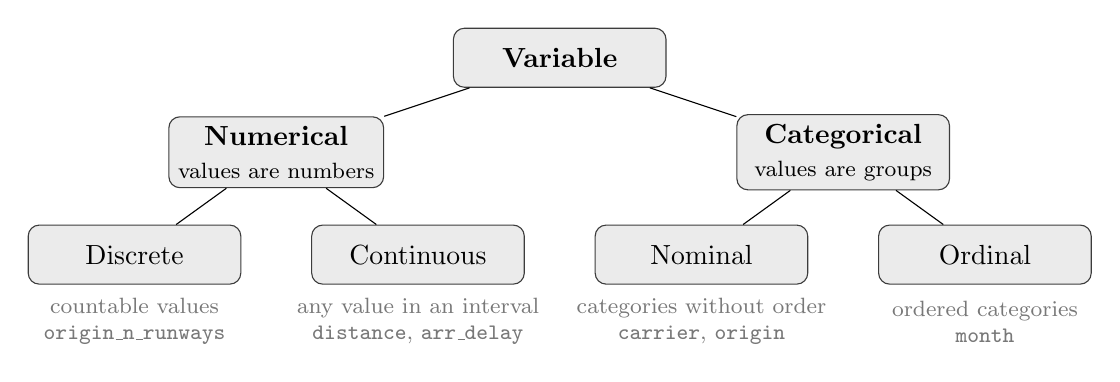
\begin{tikzpicture}[
  box/.style={draw=PelloGrayDark, rounded corners, fill=PelloGrayLight, align=center, minimum width=2.7cm, minimum height=0.75cm},
  ex/.style={align=center, font=\footnotesize, text=PelloGray}]
  \node[box] (var) at (0,0) {\textbf{Variable}};
  \node[box] (num) at (-3.6,-1.2) {\textbf{Numerical}\\ \footnotesize values are numbers};
  \node[box] (cat) at (3.6,-1.2) {\textbf{Categorical}\\ \footnotesize values are groups};
  \node[box] (dis) at (-5.4,-2.5) {Discrete};
  \node[box] (con) at (-1.8,-2.5) {Continuous};
  \node[box] (nom) at (1.8,-2.5) {Nominal};
  \node[box] (ord) at (5.4,-2.5) {Ordinal};
  \node[ex] at (-5.4,-3.35) {countable values\\ \texttt{origin\_n\_runways}};
  \node[ex] at (-1.8,-3.35) {any value in an interval\\ \texttt{distance}, \texttt{arr\_delay}};
  \node[ex] at (1.8,-3.35) {categories without order\\ \texttt{carrier}, \texttt{origin}};
  \node[ex] at (5.4,-3.35) {ordered categories\\ \texttt{month}};
  \draw (var) -- (num); \draw (var) -- (cat);
  \draw (num) -- (dis); \draw (num) -- (con);
  \draw (cat) -- (nom); \draw (cat) -- (ord);
\end{tikzpicture}
\end{center}
\end{frame}

\begin{frame}{Types of Variables and Their Graphs}

\begin{center}
\small
\begin{tabular}{llll}
\toprule
\textbf{Graph} & \textbf{Variables} & \textbf{Shows} & \textbf{ggplot2} \\
\midrule
Histogram    & 1 continuous                 & distribution of a variable          & \texttt{geom\_histogram()} \\
Bar chart    & 1 categorical                & number of observations per category & \texttt{geom\_bar()} \\
Box plot     & 1 continuous + 1 categorical & distribution within each category   & \texttt{geom\_boxplot()} \\
Scatter plot & 2 continuous                 & relationship between two variables  & \texttt{geom\_point()} \\
Line graph   & 1 continuous + time          & evolution of a variable over time   & \texttt{geom\_line()} \\
\bottomrule
\end{tabular}
\end{center}
\end{frame}

\section{ggplot2}

\begin{frame}[fragile]{Plotting Data with ggplot2}
\linespread{1.2}\selectfont

\textbf{ggplot2} is the most widely used R package for graphs. A plot is built in \textbf{layers} joined with \texttt{+}:
\begin{itemize}
  \item \texttt{ggplot(data, aes(...))}: the dataset and which variables go on each axis (or colour, fill\dots).
  \item \texttt{geom\_...()}: the type of graph (histogram, points, lines\dots).
  \item \texttt{labs()}, \texttt{theme()}, \dots: labels and appearance.
\end{itemize}

Minimal example:

\pause
\begin{lstlisting}[language=R, basicstyle=\ttfamily\small, frame=single]
# Histogram of arrival delays
ggplot(df_flights, aes(x = arr_delay)) +
  geom_histogram(bins = 30) +
  labs(x = "Arrival delay (minutes)", y = "Frequency")
\end{lstlisting}
\pause
\begin{block}{Note}
Cancelled flights have no \texttt{arr\_delay} or \texttt{air\_time}, so ggplot warns that it removed rows with missing values. The plot is still drawn.
\end{block}

\end{frame}

% Figures built by w3_figures.R (run from the project root)
\begin{frame}[fragile]{Histogram of arrival delays}
\begin{columns}[c]
\begin{column}{0.45\textwidth}
\begin{lstlisting}[language=R, basicstyle=\ttfamily\footnotesize, frame=single]
# Histogram of arrival delays
ggplot(df_flights, aes(x = arr_delay)) +
  geom_histogram(bins = 30) +
  labs(x = "Arrival delay (minutes)",
       y = "Frequency")
\end{lstlisting}
\end{column}
\begin{column}{0.55\textwidth}
\centering
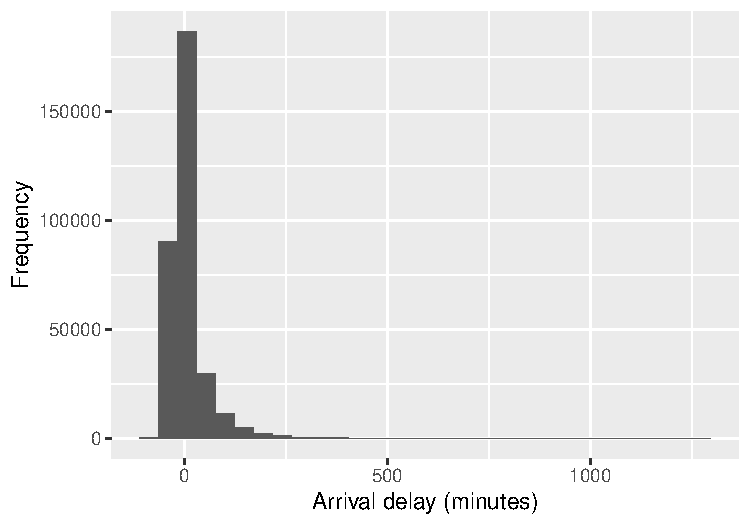
\includegraphics[width=\linewidth]{w3_hist_arr_delay.pdf}
\end{column}
\end{columns}
\end{frame}

\section{Histogram}

\begin{frame}{Histogram}
\begin{center}
  Represents the distribution of a \textbf{single continuous variable}.
\end{center}
\vspace{0.3cm}
\begin{columns}[c]
\begin{column}{0.5\textwidth}
\begin{itemize}
  \item \textbf{Horizontal axis}: the values of the variable, divided into intervals of equal width (\textbf{bins}).
  \item \textbf{Vertical axis}: the \textbf{number of observations} (frequency) whose value falls in each bin.
  \item The \textbf{height} of each bar is the count.
\end{itemize}
\end{column}
\begin{column}{0.5\textwidth}
\centering
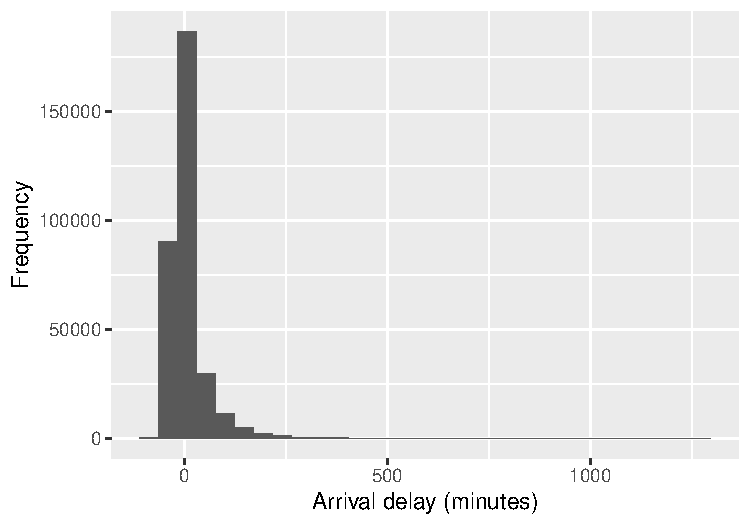
\includegraphics[width=0.8\linewidth]{w3_hist_arr_delay.pdf}
\end{column}
\end{columns}
\vfill
\vspace{0.3cm}
Decision: The number of bins (\texttt{bins = 30}) changes how detailed the shape looks.
\end{frame}

\begin{frame}{Vibecoding Graphs}
\linespread{1.4}\selectfont
  \begin{center}
    Before LLMs $\rightarrow$ graph scarcity.  After LLMs $\rightarrow$ graph congestion.
  \end{center}
  \medskip

  Think before vibecoding: what is the purpose of the graph? What is the best way to show it?

  \medskip
  \pause
  \begin{block}{}
  \textit{I am working on R using the \texttt{ggplot2} graphs package. I have a continuous variable \texttt{df\_flights\$arr\_delay}, representing the arrival delay of flights that departed from NYC airports. The dataset is based on the "flights" dataset from the \texttt{nycflights13} R package. Write an R script using ggplot2 that shows a histogram of this variable.}
  \end{block}
  \pause
  \begin{itemize}
    \item The programming language, the package.
    \item The dataset and variable names.
    \item The type of graph.
  \end{itemize}
  
\end{frame}

\begin{frame}[fragile]{First Attempt}
\begin{columns}[c]
\begin{column}{0.5\textwidth}
\begin{lstlisting}[language=R, basicstyle=\ttfamily\scriptsize]
library(ggplot2)

ggplot(df_flights, aes(x = arr_delay)) +
  geom_histogram(binwidth = 10,
                 fill = "steelblue",
                 color = "white",
                 na.rm = TRUE) +
  labs(title = "Distribution of Arrival Delays",
       x = "Arrival delay (minutes)",
       y = "Number of flights") +
  theme_minimal()
\end{lstlisting}
\end{column}
\begin{column}{0.5\textwidth}
\centering
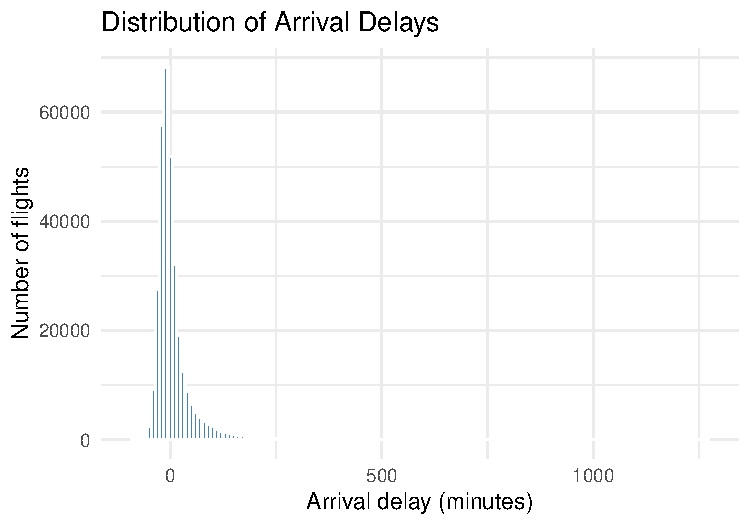
\includegraphics[width=\linewidth]{w3_vibe_hist_1.pdf}
\end{column}
\end{columns}
\pause
\vspace{0.3cm}
\begin{center}
  How would you improve this histogram?
\end{center}
\end{frame}

\begin{frame}[fragile]{Refining the Histogram}

  \begin{block}{}
  \textit{I want to improve the histogram of arrival delays. I want to reduce the horizontal axis range to a maximum of 300 minutes. Add a footnote that explains this axis range limitation.}
  \end{block}
  \vspace{0,2cm}
\begin{columns}[c]
\begin{column}{0.5\textwidth}
\begin{lstlisting}[language=R, basicstyle=\ttfamily\scriptsize]
n_above <- sum(df_flights$arr_delay > 300,
               na.rm = TRUE)

ggplot(df_flights, aes(x = arr_delay)) +
  geom_histogram(binwidth = 10,
                 fill = "steelblue",
                 color = "white",
                 na.rm = TRUE) +
  coord_cartesian(xlim = c(NA, 300)) +
  labs(title = "Distribution of Arrival Delays",
       x = "Arrival delay (minutes)",
       y = "Number of flights",
       caption = paste0(
         "Note: horizontal axis limited to 300 ",
         "minutes. ", n_above, " flights with ",
         "longer delays are not shown.")) +
  theme_minimal()
\end{lstlisting}
\end{column}
\begin{column}{0.5\textwidth}
\centering
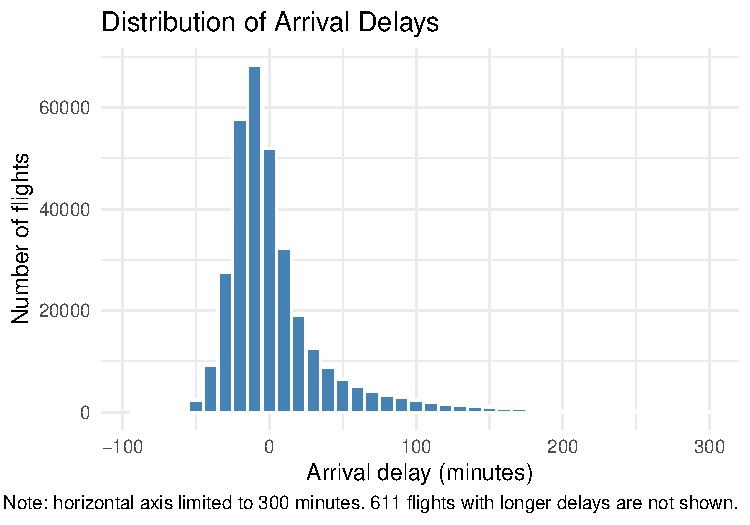
\includegraphics[width=\linewidth]{w3_vibe_hist_2.pdf}
\end{column}
\end{columns}
\end{frame}

\section{Bar Chart}

\begin{frame}[fragile]{Bar Chart}
\begin{center}
  Represents the frequency of a \textbf{single categorical variable}.
\end{center}
\vspace{0.3cm}
\begin{columns}[c]
\begin{column}{0.5\textwidth}
\begin{overprint}
\onslide<1>
\begin{itemize}
  \item \textbf{Horizontal axis}: the categories of the variable (months of the year), one bar per category.
  \item \textbf{Vertical axis}: the \textbf{number of observations} in each category.
  \item The \textbf{height} of each bar is the observation count.
\end{itemize}
\onslide<2>
\begin{lstlisting}[language=R, basicstyle=\ttfamily\footnotesize, frame=single]
# Bar chart of flights per month
ggplot(df_flights,
       aes(x = factor(month))) +
  geom_bar() +
  labs(x = "Month",
       y = "Number of flights")
\end{lstlisting}
\end{overprint}
\end{column}
\begin{column}{0.5\textwidth}
\centering
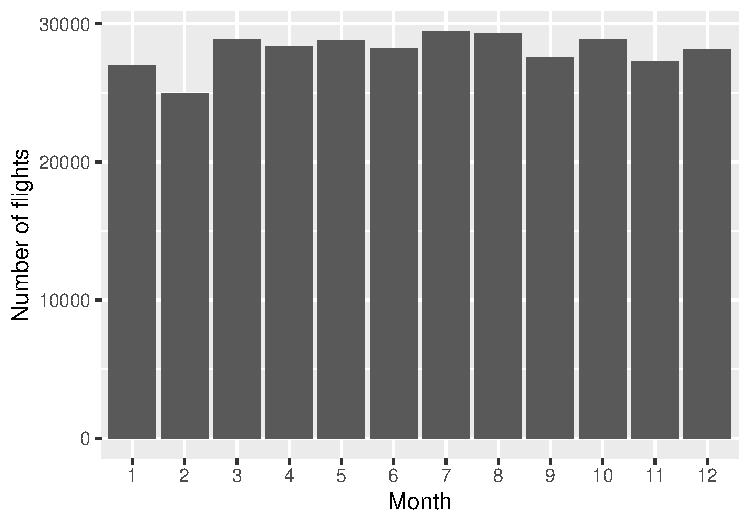
\includegraphics[width=0.8\linewidth]{w3_bar_month.pdf}
\end{column}
\end{columns}
\end{frame}

\begin{frame}[fragile]{Bar Chart: Adding Categories with Colours}
\linespread{1.2}\selectfont
A \textbf{second categorical variable} can be shown with the \textbf{colour} of the bars.
\begin{columns}[c]
\begin{column}{0.5\textwidth}
\begin{itemize}
  \item One colour per airport, shown in the \textbf{legend}.
  \item Each colour counts the flights in a month \textbf{and} from one airport.
  \item Decision: bars can be \textbf{side by side} or \textbf{stacked}.
\end{itemize}
\begin{overprint}
\onslide<1>
\begin{lstlisting}[language=R, basicstyle=\ttfamily\footnotesize, frame=single]
# Stacked (default)
ggplot(df_flights,
       aes(x = factor(month),
           fill = origin)) +
  geom_bar() +
  labs(x = "Month",
       y = "Number of flights",
       fill = "Origin")
\end{lstlisting}
\onslide<2>
\begin{lstlisting}[language=R, basicstyle=\ttfamily\footnotesize, frame=single]
# Side by side
ggplot(df_flights,
       aes(x = factor(month),
           fill = origin)) +
  geom_bar(position = "dodge") +
  labs(x = "Month",
       y = "Number of flights",
       fill = "Origin")
\end{lstlisting}
\end{overprint}
\end{column}
\begin{column}{0.5\textwidth}
\centering
\only<1>{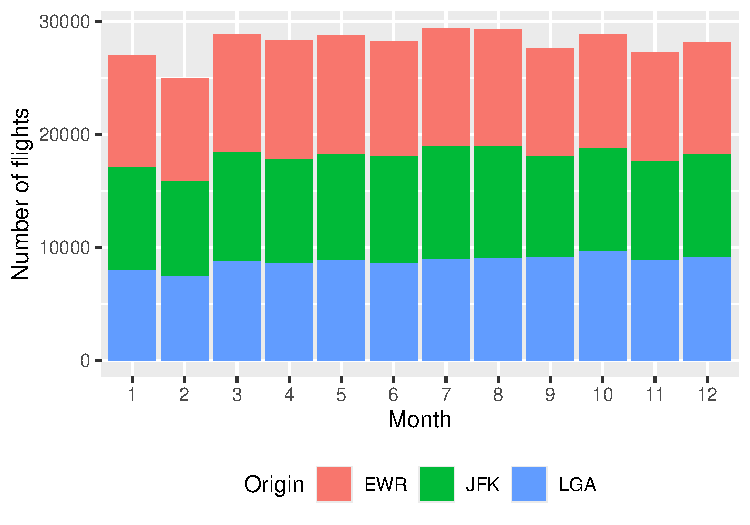
\includegraphics[width=0.9\linewidth]{w3_bar_month_origin_stack.pdf}}%
\only<2>{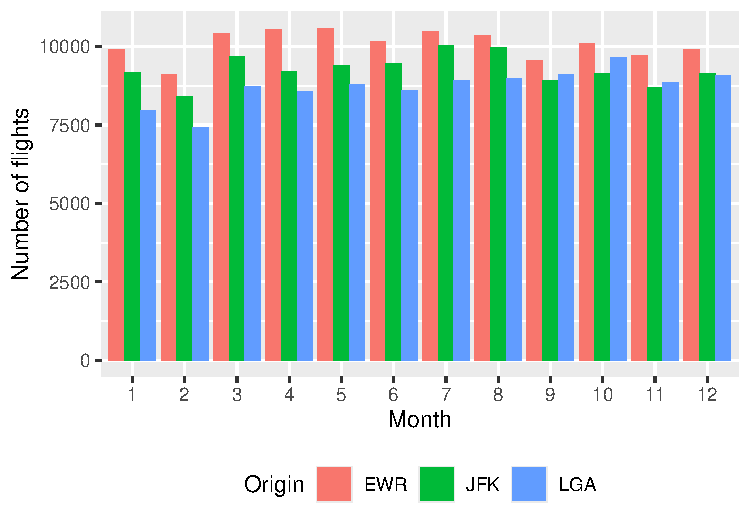
\includegraphics[width=0.9\linewidth]{w3_bar_month_origin.pdf}}
\end{column}
\end{columns}
\end{frame}

\begin{frame}{Bar Chart Type Discussion}
\linespread{1.2}\selectfont
\begin{columns}[t]
\begin{column}{0.5\textwidth}
\centering
\textbf{Stacked} (default)\\[0.3em]
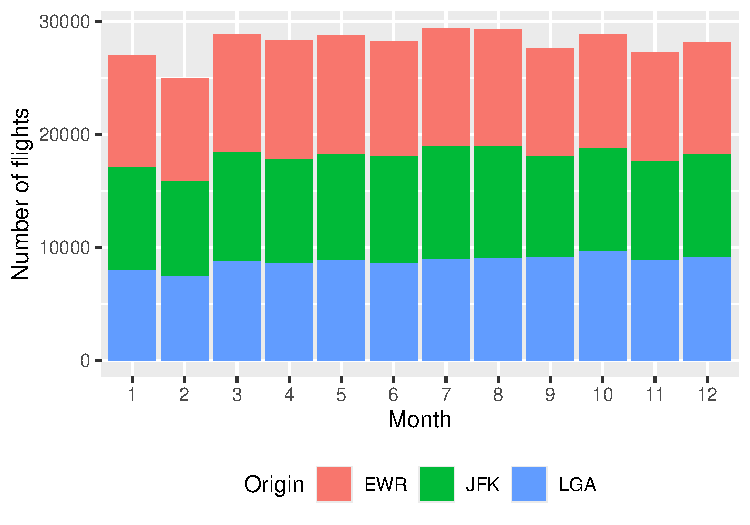
\includegraphics[width=0.85\linewidth]{w3_bar_month_origin_stack.pdf}
\end{column}
\begin{column}{0.5\textwidth}
\centering
\textbf{Side by side} (\texttt{position = "dodge"})\\[0.3em]
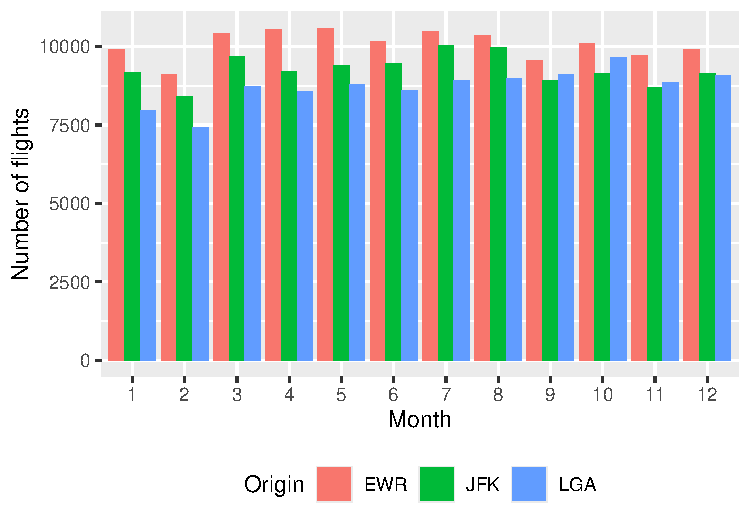
\includegraphics[width=0.85\linewidth]{w3_bar_month_origin.pdf}
\end{column}
\end{columns}
\vfill
\begin{center}
Which do you prefer? Why?
\end{center}
\end{frame}

\section{Box Plot}

\begin{frame}{Box Plot}
\linespread{1.15}\selectfont
\begin{center}
  Summary statistics of a \textbf{continuous variable} (delay time) within each \textbf{category} (airport of origin).
\end{center}
\vspace{0.3cm}
\begin{columns}[c]
\begin{column}{0.5\textwidth}
\begin{itemize}
  \item \textbf{Horizontal axis}: the categories of the variable.
  \item \textbf{Vertical axis}: continuous variable.
  \item The \textbf{line} inside the box is the median.
  \item The \textbf{box} ranges from the 25th to the 75th percentile.
  \item The \textbf{whiskers} extend to the most extreme values that lie within 1.5 box heights. \pause
  \item \textbf{Points} outside the whiskers.
\end{itemize}
\end{column}
\begin{column}{0.5\textwidth}
\centering
\only<1>{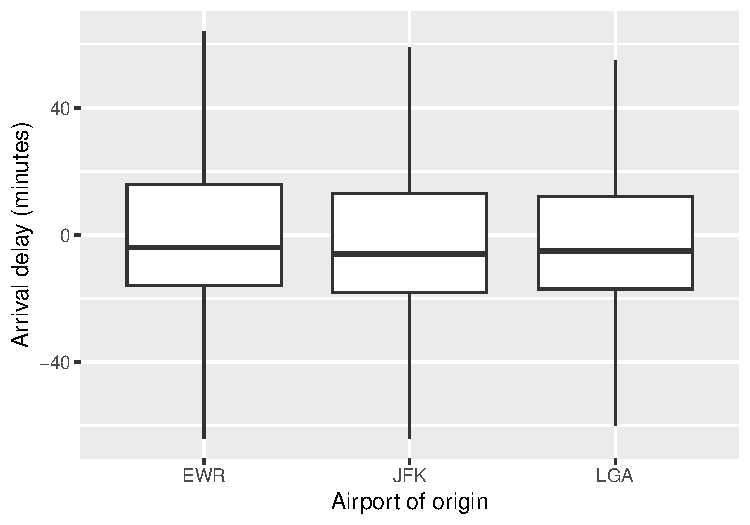
\includegraphics[width=0.8\linewidth]{w3_box_origin_nooutliers.pdf}}%
\only<2->{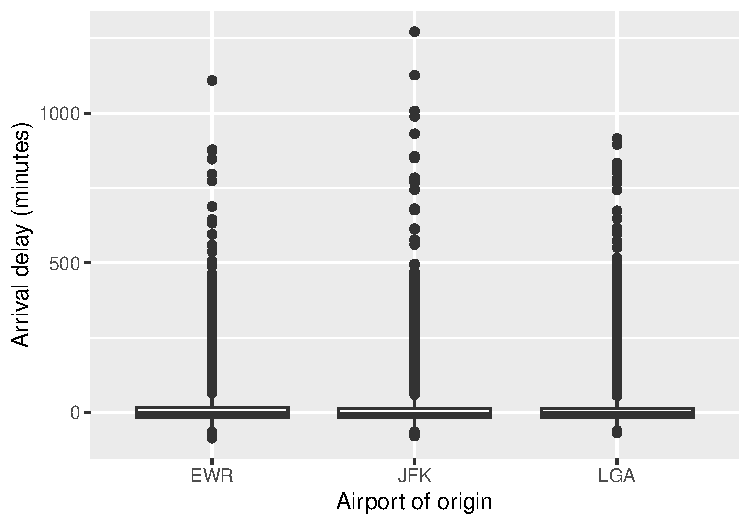
\includegraphics[width=0.8\linewidth]{w3_box_origin.pdf}}
\end{column}
\end{columns}
\pause
\vspace{0.5cm}
Decision: should we include outliers?
\end{frame}

\begin{frame}{Box Plot: Adding Categories with Colours}
\linespread{1.2}\selectfont
\begin{center}
  A \textbf{second categorical variable} (month of the year) can be shown with the \textbf{colour} of the boxes.
\end{center}
\vspace{0.3cm}
\begin{columns}[c]
\begin{column}{0.5\textwidth}
\begin{itemize}
  \item One colour per month of the year, shown in the \textbf{legend}.
  \item Within each airport, the boxes of each month are placed \textbf{side by side}.
  \item Each box summarises the delays of the flights from one airport \textbf{and} in one month.
  \item With 12 categories, that is 36 boxes: hard to read and to compare.
\end{itemize}
\end{column}
\begin{column}{0.5\textwidth}
\centering
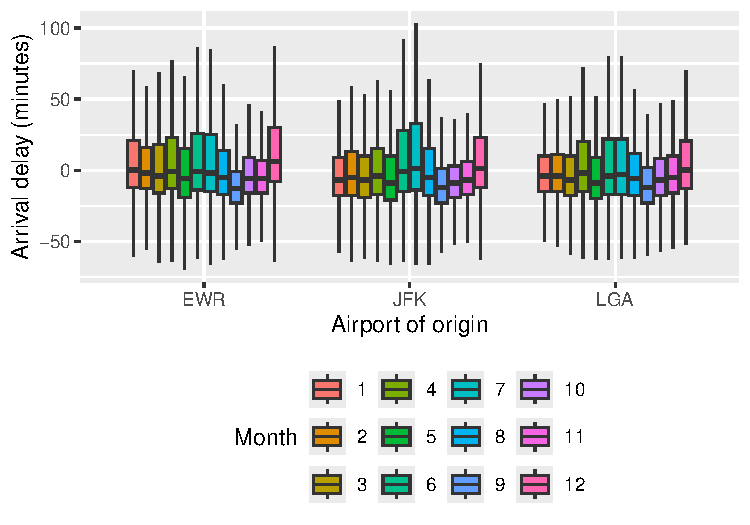
\includegraphics[width=0.8\linewidth]{w3_box_origin_month.pdf}
\end{column}
\end{columns}
\vspace{0.5cm}
\pause
What does the graph show? How can we improve it?
\end{frame}

\section{Scatter Plot}

\begin{frame}[fragile]{Scatter Plot}
\linespread{1.2}\selectfont
\begin{center}
  Represents the correlation between \textbf{two continuous variables} (distance and arrival delay).
\end{center}
\vspace{0.3cm}
\begin{columns}[c]
\begin{column}{0.5\textwidth}
\begin{overprint}
\onslide<1>
\begin{itemize}
  \item \textbf{Horizontal axis}: the first continuous variable (distance in miles).
  \item \textbf{Vertical axis}: the second continuous variable (arrival delay in minutes).
  \item Each \textbf{point} is one observation (one flight), placed at its distance and its delay.
  \item With many observations, points overlap: transparency (\texttt{alpha = 0.2}) shows where they concentrate.
\end{itemize}
\onslide<2->
\begin{lstlisting}[language=R, basicstyle=\ttfamily\footnotesize, frame=single]
# Scatter plot of delay against distance
ggplot(df_flights,
       aes(x = distance,
           y = arr_delay)) +
  geom_point(alpha = 0.2) +
  labs(x = "Distance (miles)",
       y = "Arrival delay (minutes)")
\end{lstlisting}
\begin{center}
  What does the plot show?
\end{center}
\end{overprint}
\end{column}
\begin{column}{0.5\textwidth}
\centering
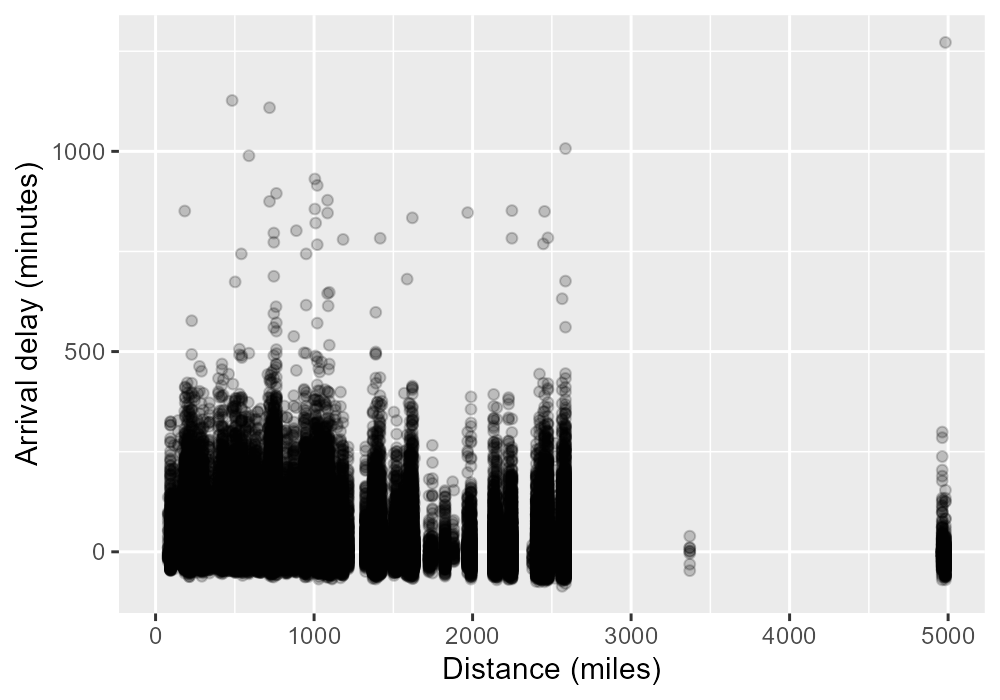
\includegraphics[width=0.8\linewidth]{w3_scatter_distance_delay.png}
\end{column}
\end{columns}

\end{frame}

\begin{frame}{Binscatter Plot}
\linespread{1.2}\selectfont
\begin{center}
  When scatterplots are too crowded, they can be summarized with a binscatter plot.
\end{center}
\vspace{0.3cm}
\begin{columns}[c]
\begin{column}{0.5\textwidth}
\begin{itemize}
  \item \textbf{Horizontal axis}: the first variable (distance), divided into 20 \textbf{bins} with the same number of flights each.
  \item \textbf{Vertical axis}: the \textbf{mean} of the second variable (arrival delay) within each bin.
  \item Each \textbf{point} is one bin, not one flight.
\end{itemize}
\end{column}
\begin{column}{0.5\textwidth}
\centering
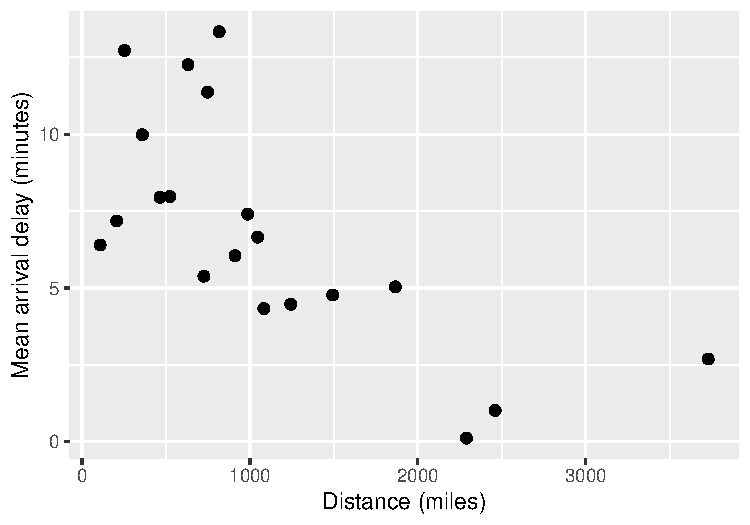
\includegraphics[width=0.8\linewidth]{w3_binscatter_distance_delay.pdf}
\end{column}
\end{columns}
\vfill
\vspace{0.3cm}
\begin{center}
  The hidden pattern \textbf{emerges}: longer flights arrive, on average, with shorter delays.
\end{center}
\end{frame}

\begin{frame}[fragile]{Vibecoding a Binscatter Plot}
\linespread{1.2}\selectfont

 \begin{block}{}
  \textit{I have this scatterplot that is too crowded [paste the previous code here]. I want to turn it into a binscatter plot with 20 bins. Please reflect any other arbitrary decisions in the graph footnote.}
  \end{block}
  \pause
\begin{columns}[c]
\begin{column}{0.55\textwidth}
\begin{lstlisting}[language=R, basicstyle=\ttfamily\scriptsize, frame=single]
d <- subset(df_flights, !is.na(arr_delay))
brk <- quantile(d$distance,
                probs = seq(0, 1, 0.05))
d$bin <- cut(d$distance, unique(brk),
             include.lowest = TRUE)
bins <- aggregate(cbind(distance, arr_delay)
                  ~ bin, data = d, FUN = mean)
\end{lstlisting}
\begin{lstlisting}[language=R, basicstyle=\ttfamily\scriptsize, frame=single]
ggplot(bins, aes(x = distance,
                 y = arr_delay)) +
  geom_point(size = 2) +
  labs(x = "Distance (miles)",
       y = "Mean arrival delay (minutes)",
       caption = paste(
         "Note: 20 distance bins with roughly equal",
         "numbers of flights. Points are bin means.",
         "Cancelled flights (no delay) excluded.",
         sep = "\n"))
\end{lstlisting}
\end{column}
\begin{column}{0.45\textwidth}
\only<2>{%
\linespread{1.1}\selectfont\footnotesize
\textbf{How the bins are made:}
\begin{enumerate}
  \item Order the flights by distance, drop \texttt{NA} values.
  \item \texttt{brk} breaks at every 5th percentile.
  \item \texttt{d\$bin} assigns each flight to one of the 20 bins.
  \item \texttt{bins} computes the mean distance and the mean delay.
\end{enumerate}}%
\only<3>{%
\centering
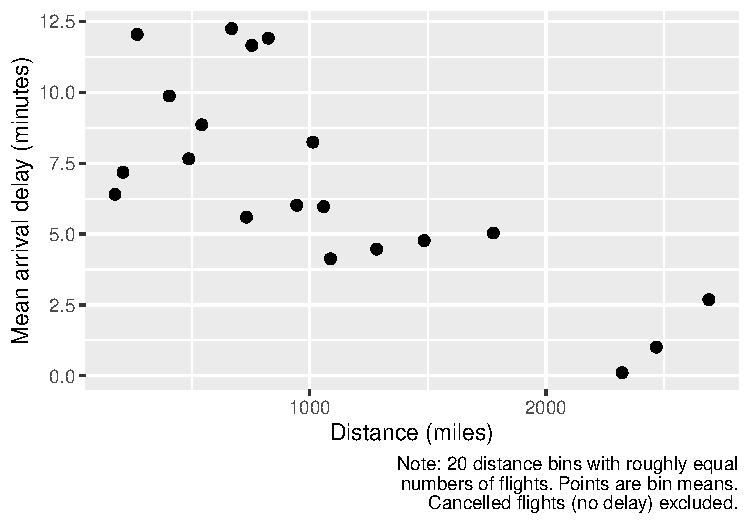
\includegraphics[width=0.9\linewidth]{w3_vibe_binscatter.pdf}}
\end{column}
\end{columns}
\end{frame}

\begin{frame}[fragile]{Binscatter improvements: Adding Categories with Colours}
\linespread{1.2}\selectfont

 \begin{block}{}
  \textit{Can you improve the previous binscatter by classifying the flights by their origin airport? Each airport should be represented by a different colour. Please add a legend to the graph.}
  \end{block}
  \pause
\begin{columns}[c]
\begin{column}{0.55\textwidth}
\begin{lstlisting}[language=R, basicstyle=\ttfamily\scriptsize, frame=single]
# Same bins as before (d, brk, d$bin)
bins <- aggregate(cbind(distance, arr_delay)
                  ~ bin + origin,
                  data = d, FUN = mean)
\end{lstlisting}
\begin{lstlisting}[language=R, basicstyle=\ttfamily\scriptsize, frame=single]
ggplot(bins, aes(x = distance,
                 y = arr_delay,
                 colour = origin)) +
  geom_point(size = 2) +
  labs(x = "Distance (miles)",
       y = "Mean arrival delay (minutes)",
       colour = "Origin",
       caption = paste(
         "Note: same 20 distance bins for all airports.",
         "Points are bin means for each airport.",
         "Cancelled flights (no delay) excluded.",
         sep = "\n"))
\end{lstlisting}
\end{column}
\begin{column}{0.45\textwidth}
\centering
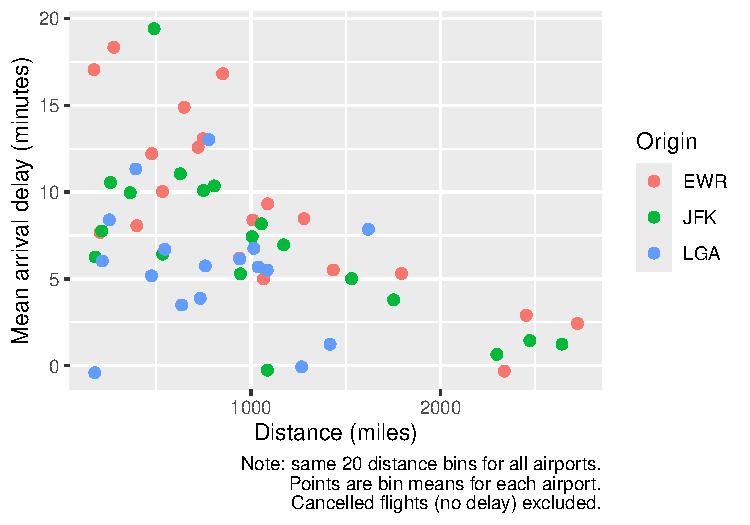
\includegraphics[width=0.9\linewidth]{w3_vibe_binscatter_origin.pdf}
\end{column}
\end{columns}
\end{frame}



\section{Line Graph}

\begin{frame}[fragile]{Line Graph}
\linespread{1.2}\selectfont
\begin{center}
  A line graph shows how \textbf{one continuous variable evolves over time}.
\end{center}
\vspace{0.2cm}
\begin{columns}[c]
\begin{column}{0.5\textwidth}
\begin{overprint}
\onslide<1>
\begin{itemize}
  \item \textbf{Horizontal axis}: time (here, each day of 2013).
  \item \textbf{Vertical axis}: the value of the variable at each date (here, the number of flights that day).
  \item Points are \textbf{connected in time order}.
\end{itemize}
\onslide<2>
\begin{lstlisting}[language=R, basicstyle=\ttfamily\scriptsize, frame=single]
# Count the flights of each day
library(dplyr)
daily <- df_flights |>
  mutate(date = as.Date(paste(year, month,
                              day, sep = "-"))) |>
  group_by(date) |>
  summarise(n = n())
\end{lstlisting}
\begin{lstlisting}[language=R, basicstyle=\ttfamily\scriptsize, frame=single]
ggplot(daily, aes(x = date, y = n)) +
  geom_line() +
  labs(x = "Date", y = "Number of flights")
\end{lstlisting}
\end{overprint}
\end{column}
\begin{column}{0.5\textwidth}
\centering
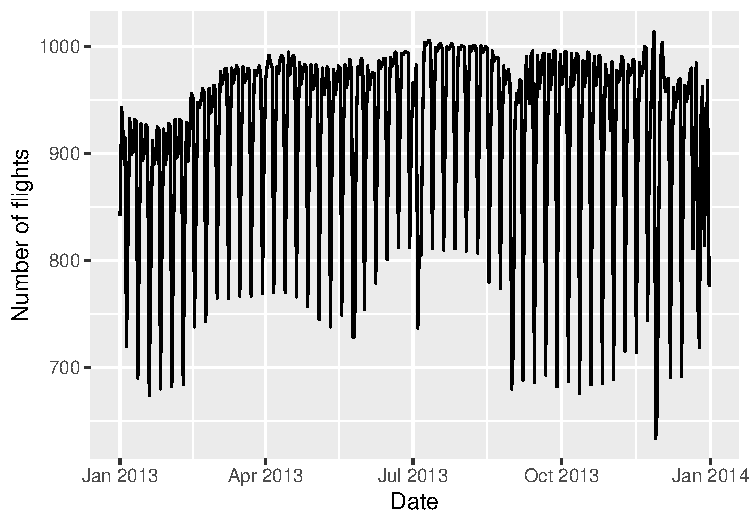
\includegraphics[width=0.85\linewidth]{w3_line_daily.pdf}
\end{column}
\end{columns}

\begin{center}
  What does the graph show? How can we improve it?
\end{center}

\end{frame}

\begin{frame}[fragile]{Line Graph: Aggregating to Months}
\linespread{1.2}\selectfont
\begin{center}
  The \textbf{time unit} we choose changes what the graph shows.
\end{center}
\vspace{0.2cm}
\begin{columns}[c]
\begin{column}{0.5\textwidth}
\begin{lstlisting}[language=R, basicstyle=\ttfamily\scriptsize, frame=single]
# Count the flights of each month
df_flights <- df_flights |>
  mutate(ym = as.Date(paste(year, month,
                            1, sep = "-")))
monthly <- df_flights |>
  group_by(ym) |>
  summarise(n = n())
\end{lstlisting}
\begin{lstlisting}[language=R, basicstyle=\ttfamily\scriptsize, frame=single]
ggplot(monthly, aes(x = ym, y = n)) +
  geom_line() +
  geom_point() +
  scale_x_date(date_breaks = "1 month",
               date_labels = "%b") +
  labs(x = "Month", y = "Number of flights")
\end{lstlisting}
\end{column}
\begin{column}{0.5\textwidth}
\centering
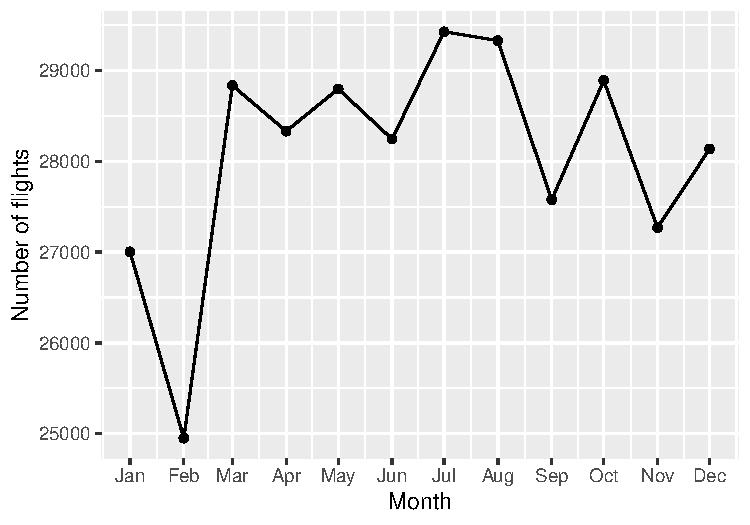
\includegraphics[width=0.85\linewidth]{w3_line_monthly.pdf}
\end{column}
\end{columns}
\begin{center}
  What is happening in February?
\end{center}
\end{frame}

\begin{frame}[fragile]{Line Graph: Starting the Vertical Axis at Zero}
\linespread{1.2}\selectfont
\begin{center}
  Where the vertical axis starts changes how \textbf{large} the changes look.
\end{center}
\vspace{0.2cm}
\begin{columns}[c]
\begin{column}{0.5\textwidth}
\begin{lstlisting}[language=R, basicstyle=\ttfamily\scriptsize, frame=single]
# Same monthly graph, vertical axis from zero
ggplot(monthly, aes(x = ym, y = n)) +
  geom_line() +
  geom_point() +
  expand_limits(y = 0) +
  scale_x_date(date_breaks = "1 month",
               date_labels = "%b") +
  labs(x = "Month", y = "Number of flights")
\end{lstlisting}
%By default, \texttt{ggplot2} zooms the vertical axis on the data, so small changes look dramatic. Starting at \textbf{zero} shows their true size: every month has between 25,000 and 29,500 flights.
\end{column}
\begin{column}{0.5\textwidth}
\centering
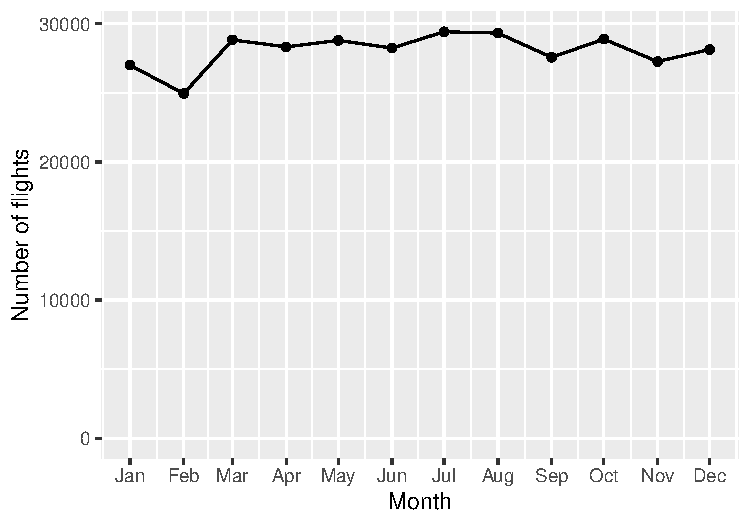
\includegraphics[width=0.85\linewidth]{w3_line_monthly_zero.pdf}
\end{column}
\end{columns}
\end{frame}

\begin{frame}[fragile]{Line Graph: Adding Categories with Colours}
\linespread{1.2}\selectfont
\begin{center}
  A \textbf{categorical variable} can be shown with one line per category.
\end{center}
\vspace{0.2cm}
\begin{columns}[c]
\begin{column}{0.5\textwidth}
\begin{lstlisting}[language=R, basicstyle=\ttfamily\scriptsize, frame=single]
# Count the flights of each month and airport
monthly_origin <- df_flights |>
  group_by(ym, origin) |>
  summarise(n = n())
\end{lstlisting}
\begin{lstlisting}[language=R, basicstyle=\ttfamily\scriptsize, frame=single]
ggplot(monthly_origin, aes(x = ym, y = n,
                           colour = origin)) +
  geom_line() +
  geom_point() +
  expand_limits(y = 0) +
  scale_x_date(date_breaks = "1 month",
               date_labels = "%b") +
  labs(x = "Month", y = "Number of flights",
       colour = "Origin") +
  theme(legend.position = "bottom")
\end{lstlisting}
\end{column}
\begin{column}{0.5\textwidth}
\centering
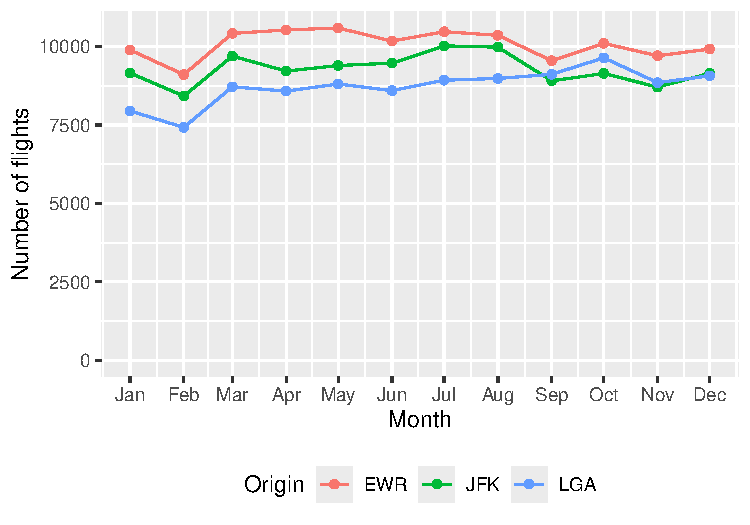
\includegraphics[width=0.85\linewidth]{w3_line_monthly_origin.pdf}
\end{column}
\end{columns}
\end{frame}

\begin{frame}[fragile]{Vibecoding a Line Graph}
\linespread{1.0}\selectfont
  \begin{block}{}
  \footnotesize\textit{I want to represent how the number of flights in each airport has changed over the months. For that, I want to aggregate the data to weekly level, then determine the first period as level 100 for each airport, and finally plot the percentage change of flights with respect to the baseline.}
  \end{block}
  \pause
\begin{columns}[c]
\begin{column}{0.55\textwidth}
\begin{lstlisting}[language=R, basicstyle=\ttfamily\tiny, frame=single]
weekly <- df_flights |>
  # week = date of the Monday that starts each week
  mutate(date = as.Date(paste(year, month, day, sep = "-")),
         week = as.Date(cut(date, "week"))) |>
  group_by(origin, week) |>
  summarise(n = n(), days = n_distinct(date), .groups = "drop") |>
  # drop incomplete weeks (start and end of the year)
  filter(days == 7) |>
  group_by(origin) |>
  mutate(index = 100 * n / first(n),
         pct_change = index - 100) |>
  ungroup()
\end{lstlisting}
\begin{lstlisting}[language=R, basicstyle=\ttfamily\scriptsize, frame=single]
ggplot(weekly, aes(x = week, y = pct_change, colour = origin)) +
  geom_hline(yintercept = 0, linetype = "dashed") +
  geom_line() + geom_point(size = 1) +
  scale_x_date(date_breaks = "1 month", date_labels = "%b") +
  labs(x = "Week", y = "Change in flights (%)", colour = "Origin",
       caption = paste("Note: first full week of 2013 = 100.",
                       "Incomplete weeks excluded."))
\end{lstlisting}
\end{column}
\begin{column}{0.45\textwidth}
\centering
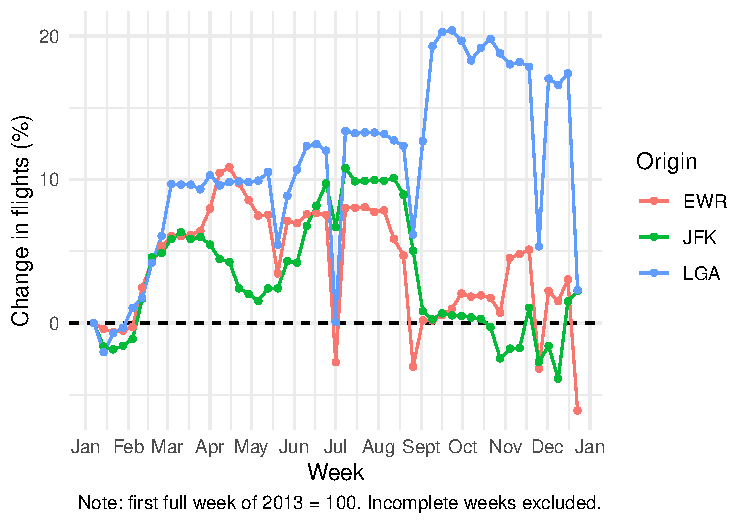
\includegraphics[width=0.95\linewidth]{w3_vibe_line_weekly.pdf}
\end{column}
\end{columns}
\end{frame}



\section{Maps}

\begin{frame}[fragile]{Maps}
\linespread{1.3}\selectfont
\textbf{One variable across regions.} Each region (country, state, municipality) is a shape, coloured by the value of a variable (a \textit{choropleth} map). Shapes come as an \texttt{sf} object, plotted with \texttt{geom\_sf()}.

\begin{columns}[t]
\begin{column}{0.5\textwidth}
\centering
\begin{lstlisting}[language=R, basicstyle=\ttfamily\scriptsize]
library(sf)
library(rnaturalearth)
world <- ne_countries(returnclass = "sf")

# Map of the world
ggplot(world) +
  geom_sf()
\end{lstlisting}
\end{column}
\begin{column}{0.5\textwidth}
\centering
\begin{lstlisting}[language=R, basicstyle=\ttfamily\scriptsize]
# Countries coloured by a variable
ggplot(world, aes(fill = pop_est)) +
  geom_sf() +
  theme(legend.position = "bottom")
\end{lstlisting}
\end{column}
\end{columns}

\pause
\begin{itemize}
  \item To map your own data, merge it into the \texttt{sf} object by a region identifier: \texttt{merge(world, df, by = "iso\_a3")}.
  \item \texttt{fill} can be continuous (income) or categorical (\texttt{continent}).
\end{itemize}
\end{frame}


\section{Summary}

\begin{frame}{Graphs: Summary}

\begin{center}
\small
\begin{tabular}{llll}
\toprule
\textbf{Graph} & \textbf{Variables plotted} & \textbf{Adding categories} & \textbf{Variables with categories} \\
\midrule
Histogram    & 1 & panels (\texttt{facet\_wrap}) or \texttt{fill} & 2 \\
Bar chart    & 1 & \texttt{fill}                                  & 2 \\
Box plot     & 2 & \texttt{fill}                                  & 3 \\
Scatter plot & 2 & \texttt{colour} or \texttt{shape}              & 3 \\
Line graph   & 2 & \texttt{colour} or \texttt{linetype}           & 3 \\
\bottomrule
\end{tabular}
\end{center}

\pause
\begin{itemize}
  \item Panels (\texttt{facet\_wrap}) work with every graph, and can be combined with colours to add yet another variable.
  \item Always label the axes and state the units: \texttt{labs(x = "...", y = "...")}.
  \item Later in the course: graphs of \textbf{estimates} rather than raw data (fitted regression lines, coefficients with confidence intervals).
\end{itemize}
\end{frame}


\end{document}

